
\section{Introduction} % Sections are added in order to organize your presentation into discrete blocks, all sections and subsections are automatically output to the table of contents as an overview of the talk but NOT output in the presentation as separate slides

%------------------------------------------------

\begin{frame}
\frametitle{FoundationDB}

\begin{figure}
    \centering
    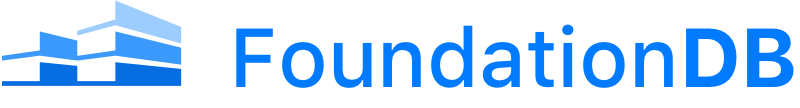
\includegraphics[width=0.5\textwidth]{img/1-Introduction/foundationBD-logo.png}
    
\end{figure}

\textbf{FoundationDB}FoundationDB is an open-source transactional key-value store created by Apple in 2009. It combine \textbf{flexibility} and \textbf{scalability} of \textbf{NoSQL} architectures with the power of \textbf{ACID transactions}.
	
\end{frame}

%------------------------------------------------

\begin{frame}
	\frametitle{FDB Key features}

Key features:
\begin{itemize}
    \item NoSQL
    \item Ordered key-value pair.
    \item Strictly serializable transactions
    \item ACID transactions
    \item Designed around Core-Layer philosophy 
    
\end{itemize}

\end{frame}
%------------------------------------------------
\begin{frame}
	\frametitle{CAP trade off}

A trade off exists between consistency, availability, and
partition tolerance
\begin{itemize}
    \item Consistency: A read sees all previously completed writes
    \item Availability: Reads and writes always succeed
    \item Partition tolerance: Guaranteed properties are maintained even when network failures prevent some machines from communicating with others.
    
\end{itemize}
FoundationBD satisfied \textbf{Consistency} and \textbf{Partition Tolerance} 

\end{frame}
%------------------------------------------------
\begin{frame}
	\frametitle{CAP Theorem Examples}

\begin{figure}[h]
    \centering
    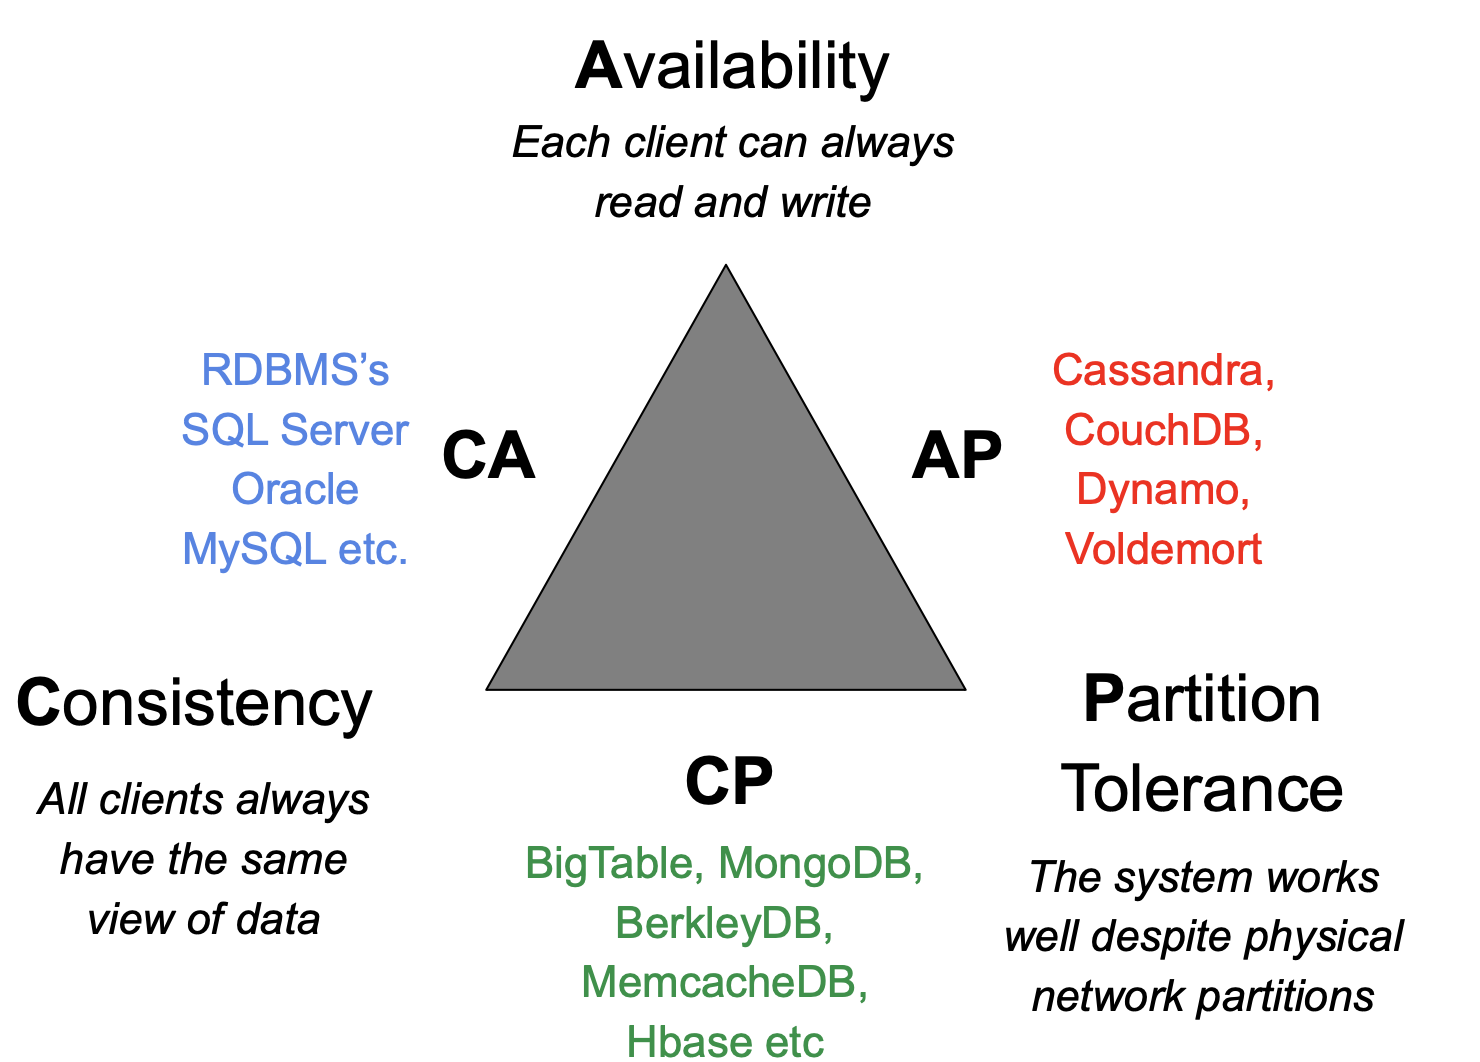
\includegraphics[width=0.7\textwidth]{img/1-Introduction/CAP theorem.png}
    \caption{CAP Theorem (or triangle)}
\end{figure}

\end{frame}
%------------------------------------------------

\begin{frame}
	\frametitle{FoundationDB approach}
Most database: 
    \begin{itemize}
        \item Storage engine
        \item Data model
        \item API/Query language
    \end{itemize}

FoundationDB has a modular approach, it it provides a highly scalable storage engine with a minimal yet carefully chosen set of features.

\vspace{0.5cm}
\begin{quote}
    \textbf{\textcolor{red}{``What features could we take away? Almost everything, we decided.''}}
\end{quote}
        
\end{frame}


%------------------------------------------------

\begin{frame}
	\frametitle{What will be discussed in the next chapters}

    \begin{itemize}
        \item Architecture of FoundationDB
        \item Simulation and Testing of distributed system
        \item Evaluation of FoundationDB
        \item Conclusions
    \end{itemize}
        
\end{frame}

%------------------------------------------------

